\section{The WODA platform}

\subsection{The workflow}
\label{generic-workflow}

The generic workflow in Figure \ref{fig:workflow_0} uses primary and authoritative data sources as an input, and iteratively augments them using computation. Wherever the conditions for computation are not verified, crowdsourcing is used to create the missing data to enable it. 

This section outlines the design principles of WODA: a re-usable platform to support implementations of such workflow. The crowdsourcing component is then explored in more detail.

\begin{figure}
	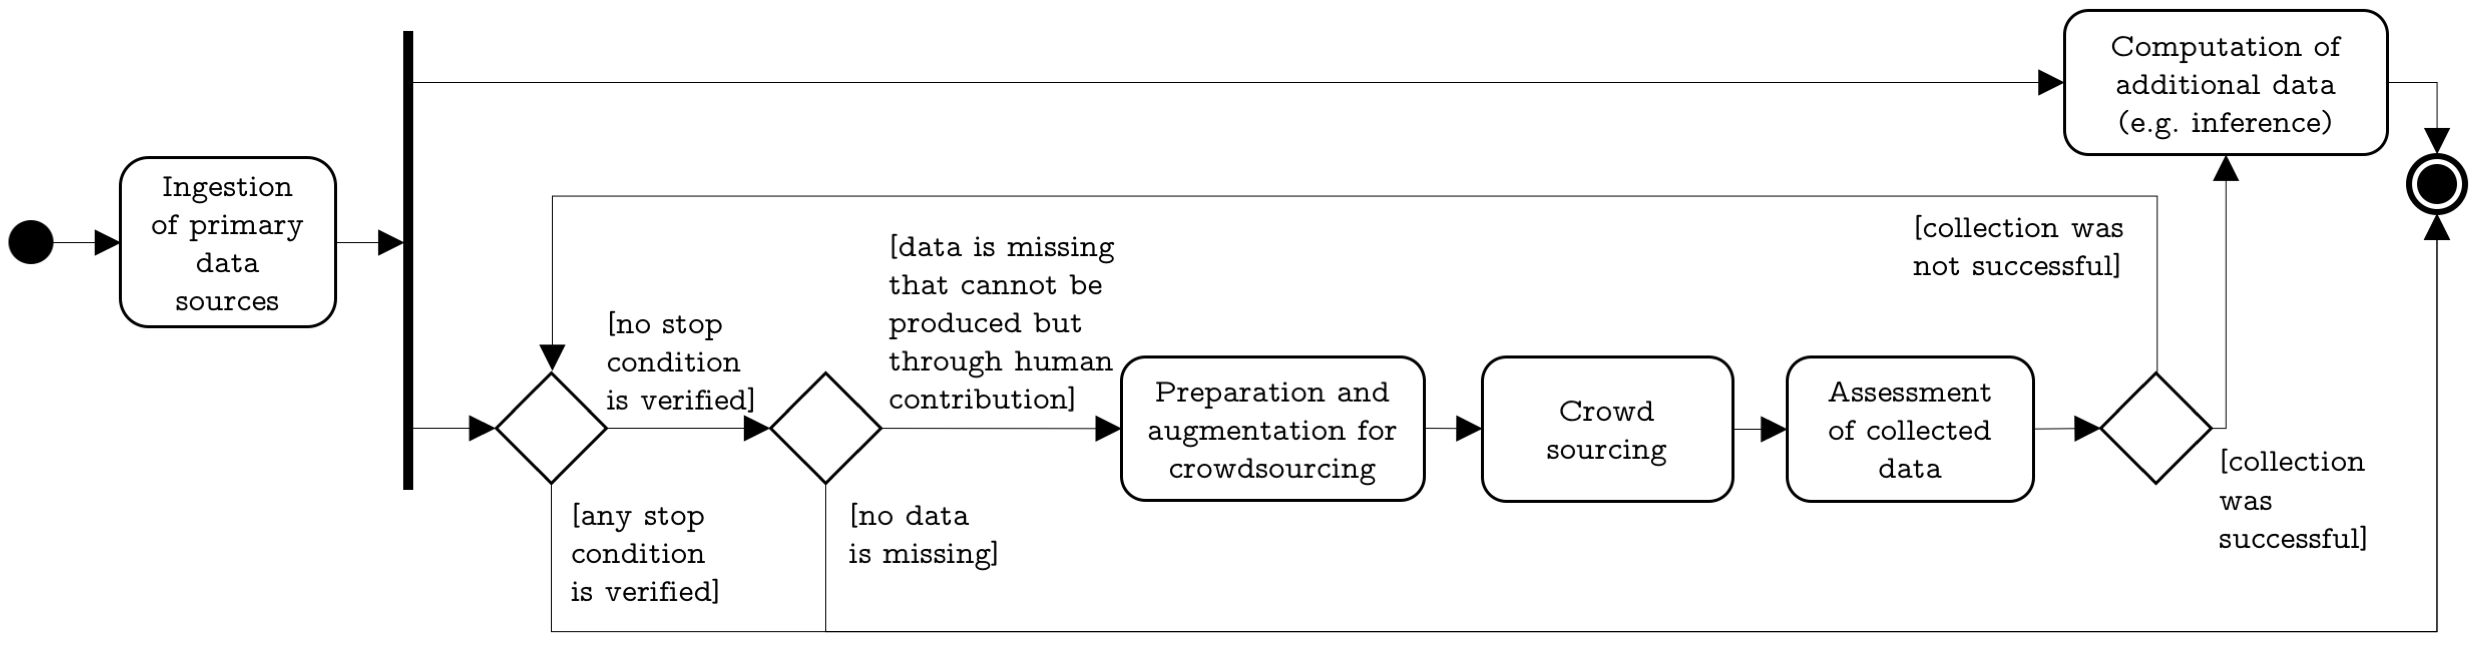
\includegraphics[width=1.0\textwidth]{workflow-0.png}
	\caption{UML process diagram of the generic WODA-supported workflow}
	\label{fig:workflow_0}
\end{figure}

\subsection{Overall design principles}
\label{desing-principles}

WODA was designed following the principles below:

\textbf{Human-machine workflows support} WODA meant to automate as much as possible of the data creation / curation process, while effectively integrating human components, from administration to the crowdsourcing of part.

\textbf{Data re-use} As mentioned in chapter \ref{open-data-and-gi} we wanted to make the best possible use of pre-existing, high quality and authoritative open data sources.

\textbf{Open source software} It was assumed that open source software could be used to implement any required component of WODA. This also saves budget for the compensation of paid contributors.

\textbf{Scalability and high availability} WODA was designed to be highly scalable and available, suitable for real-world deployment.

\textbf{Versatility} WODA had to be versatile and suitable to be applicable to a range of problems describable within the workflow above and leveraging different input data sources as needed. The crowdsourcing component is required to be flexible enough to cater for different models: paid contributors vs volunteers, approaches to results aggregation, quality assessment etc.

\subsection{Crowdsourcing design principles}

The crowdsourcing component, can be described against the dimensions presented by Simperl in \cite{Simperl:2015ju}. 

\textbf{What is outsourced} The objective of the outsourcing activity is the production of original geospatial data or the curation (correction, validation etc.) of pre-existing data, wherever the activity can be only performed by human agents. 

The activity translates into surveying the locations or examining imagery thereof and record observations (e.g. "how many trees can be seen from longitude x and latitude y?"), or amend previous recordings (e.g. "can you confirm that there is a hospital in Vicarage Rd, Watford?"). 

To avoid the cost of performing a physical survey of the locations, participants examine publicly available imagery. This is not uncommon, e.g. OSM currently uses aerial imagery from Microsoft Bing to let its contributors edit street topology.

Progress in machine learning, computer vision etc. hints at a future in which the human component may be made redundant. To this day, however, automation can only complement rather than replace humans (e.g. in \cite{Goetz:1gd} or \cite{Schmid:2012we}).

\textbf{Who is the crowd} In VGI, contributors are often associated to the locations they work on, and their work can be seen as the act of capturing the knowledge they own of a place. Occasionally, this can be instrumental to assure the completeness of the data, e.g. the function of public buildings can't be inferred from observing OSM's aerial imagery. Physical survey of the location may be also required, using specialised equipment.

To contribute to WODA, specialised knowledge, skills and equipment are not required, nor is a connection to the places being surveyed. 

\textbf{How is the task outsourced} In the current implementation, WODA focuses on outsourcing micro rather than macro tasks. Wherever possible, one's contribution is limited to a few minutes' work at the computer and does not require awareness of the larger system they are part of, in the attempt of removing complexity and barriers to participation.

\textbf{Why do people contribute} The motivation of VGI crowds is a complex subject, summarised e.g. in Coleman {\it et al.} in \cite{Coleman:2009vd}: motivation spans from altruism to intellectual stimulation, social reward and "pride of place".

In the current implementation, WODA contributors are driven merely by financial interest. They are oblivious of the the context of the project, have no personal connection to the locations, and are likely unaware of and find no motivation in contributing to the "cause" of open data. This is typically the crowd that can be recruited through mainstream crowdwork platforms. 

\subsection{Implementation}

\subsubsection{Overview} \leavevmode \\ %% Why is this necessary to get a new line?

From the \textbf{platform owner}'s point of view, WODA is made of several sets of tools to (i) ingest the primary data sources into a reference database, (ii) process the ingested data and derive new / enhanced data computationally, (iii) configure the crowdsourcing platform of choice, including the user interface participants use, (iv) support the execution of the crowdsourcing stage (load data to the crowdsourcing platform, collect its results etc.), and (v) consolidate primary, derived and crowdsourced data in one consistent dataset.

From the \textbf{participant}'s point of view, WODA presents itself simply as a task hosted on a crowdsourcing platform. The task web page offers interactive maps and panoramic views of one or more locations to survey, and a form contributors use to submit observations, as shown in Figure \ref{fig:virtual-survey-tool-01}. 

\begin{figure}
    %% NOTE: the choice of width % below is key to stay in the 18 pages limit! Even a 0.01 variation can make a difference because of how LaTeX manages text flow.
	\frame{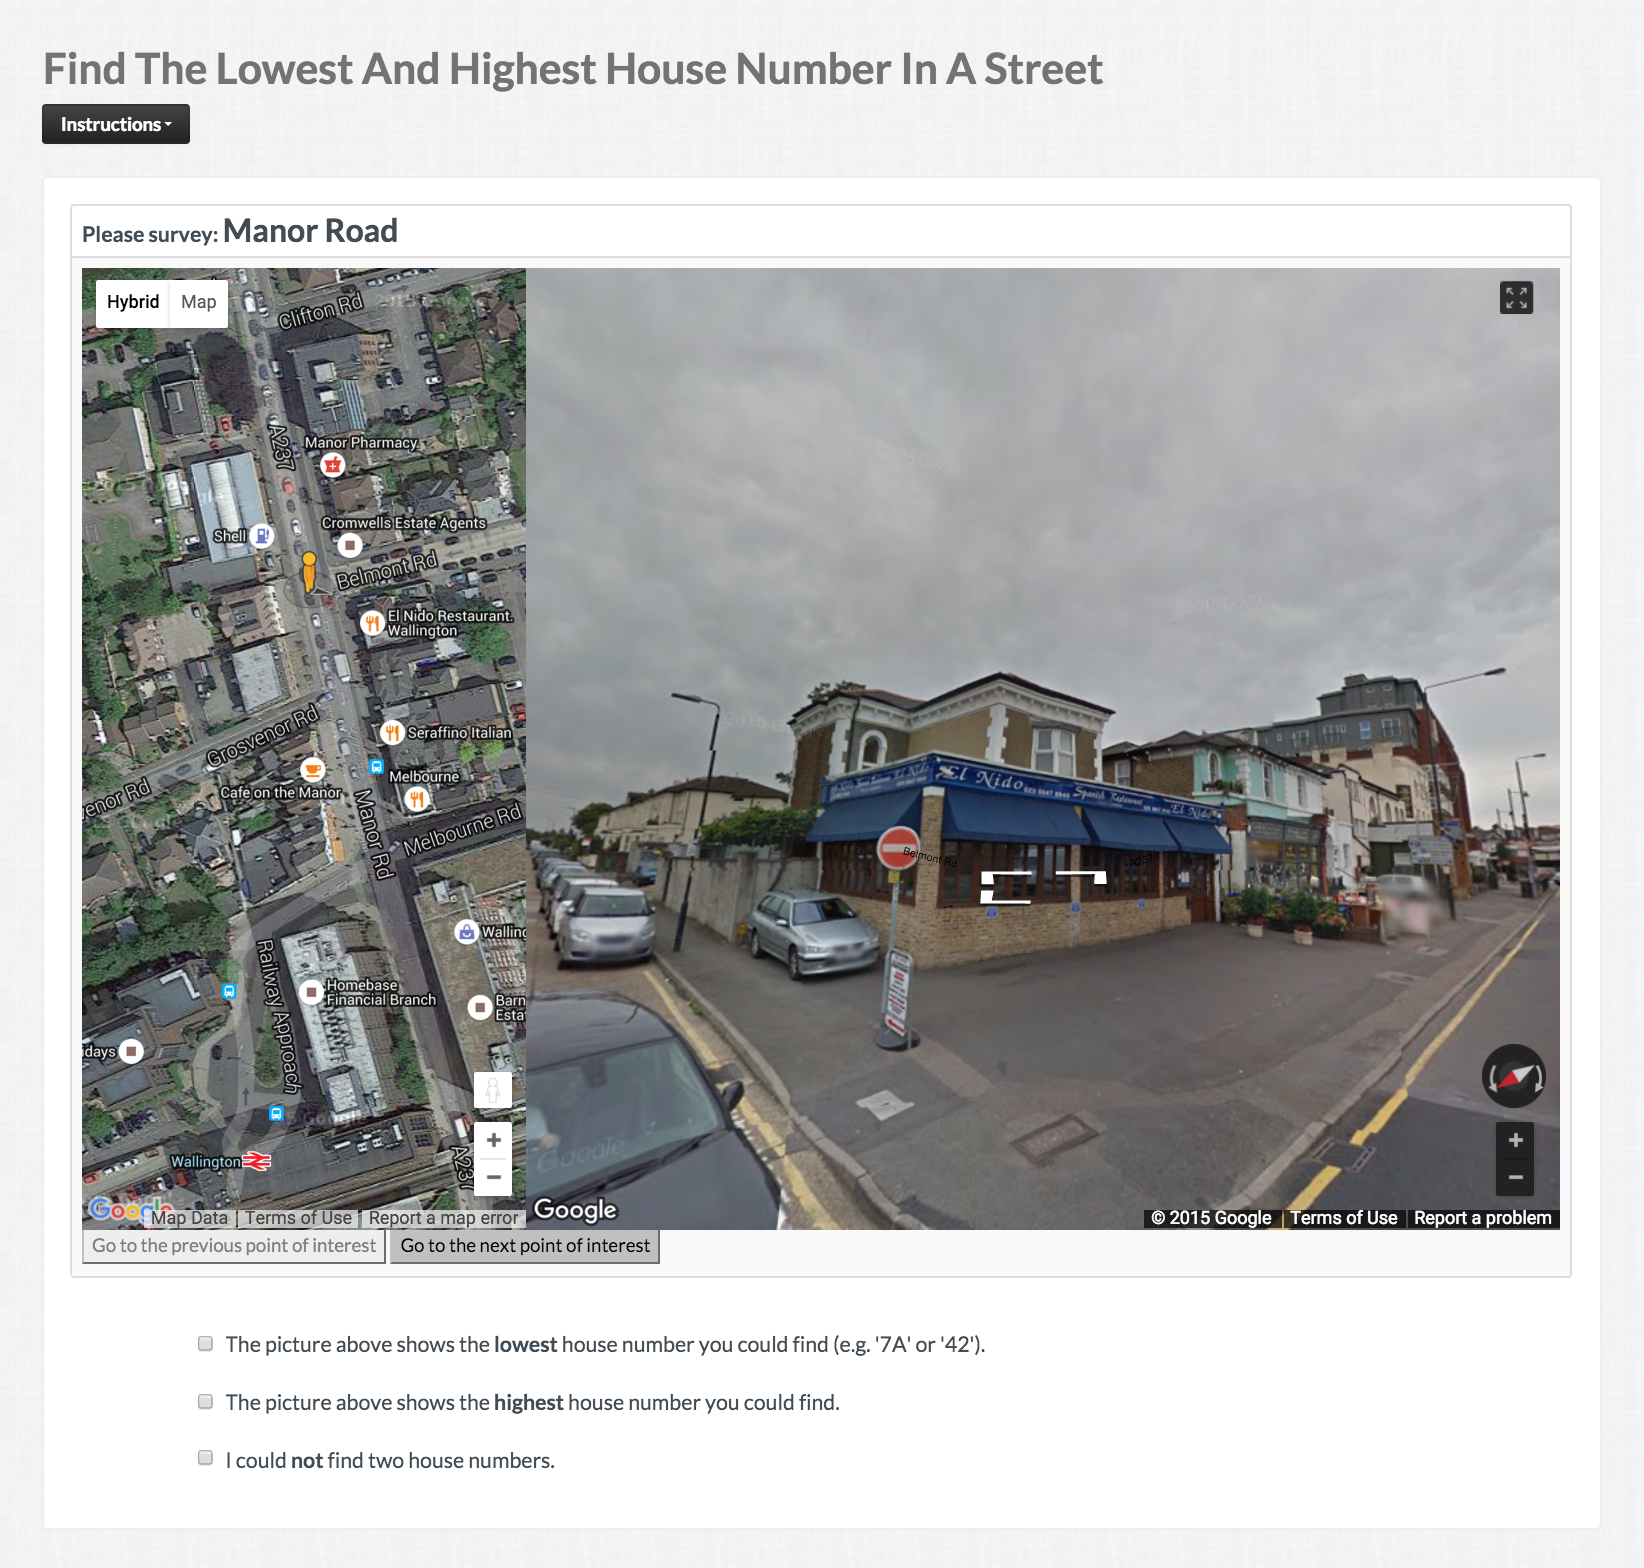
\includegraphics[width=0.69\textwidth]{virtual-survey-tool-01.png}}
	\caption{The task section of the web page, offering the Google Maps and Street View panes and the form participants use to submit their observations.}
	\label{fig:virtual-survey-tool-01}
\end{figure}

On first access, instructions are provided at the top of the page , possibly alongside a video used to illustrate the more interactive features.\footnote{See \screenshotwithvideourl.}. The video specific to OLAF's deployment of WODA can be watched at \url{https://www.youtube.com/watch?v=pIiGJ6gMEY0}.

\subsubsection{Components} \leavevmode \\ %% Why is this necessary to get a new line?

\textbf{CrowdFlower} CrowdFlower was chosen as the crowdsourcing platform. It is a SaaS specialised in hosting data-centred microtasks for volunteer or paid participants. Clients who accept that their data could be re-published as open data may access the service under a plan that has no costs but for the compensation to the paid participants and a commission. The service is available both through a templating system called CML and through APIs. 

When using CML, the options available to implement a crowdsourcing model - such as how the accuracy of the contributor is assessed or how results are aggregated - are limited by the functionality supported by the system.\footnote{For example, CrowdFlower calculates Workers' agreement as the quorum of participants who expressed the majority vote, and tasks can be stopped automatically when a target \% is achieved. The same cannot be done when using alternative statistical measures of agreement, whose calculation must take place outside the system.} In order not to introduce additional components in the system and maximise scalability and high availability, we relied on CML only and worked around its limitations by performing some of the data processing outside of CrowdFlower. 

\textbf{Google Maps} Google Maps is a mapping SaaS, made available to the public for free. It offers satellite and aerial imagery, maps, interactive panoramic views of streets alongside the metadata through APIs. Many of its services can be embedded in third party websites and customised using client-side JavaScript, hence making it suitable to integration with CrowdFlower or other template-based systems. 

\textbf{YouTube} YouTube is a video publishing platform by Google. Similarly to Google Maps, videos can be embedded in third party websites, hence is suitable for integration in CML. WODA uses YouTube to provide instructions to participants.  

\textbf{GitHub} GitHub is a web-based Git repository hosting SaaS. Together with WODA's source and documentation, it is used also for hosting static assets, e.g. the icons used to mark points of interest in Google Maps. 

\textbf{PostgreSQL + PostGIS} The PostgreSQL relational database running the PostGIS spatial extender was chosen as the main data repository. All geospatial data is converted from its source format to PostGIS' native geospatial types to be consistent across all sources and enabling geographic querying. 

\textbf{Scripting} Bash, NodeJS and PostgreSQL scripting were used to glue all components together wherever automation is possible.  

\subsection{Legal implications}

The design choices have legal implications to be taken into account when deploying beyond research.\footnote{See \url{https://peepbeep.wordpress.com/2015/12/18/what}.} It is outside of the scope of this paper to examine this in any detail, however some of the matters are described below.

\textbf{Personal data and privacy implications.} According to EU Data Protection Directive (95/46/EC), implemented in the UK by the Data Protection Act of 1998, geospatial data such as addresses can be considered as personal data even when it is not associated to information about who lives at the locations, as it is "information relating to an identified or identifiable natural person". The directive describes a framework of practices to comply with.
	
\textbf{Imagery terms and conditions} Google Maps' terms of service specify restrictions on producing "derivative works of the Content or any part thereof" and on creating "a database of places or other local listings information". It is advisable that - before deploying WODA for real-world applications - the mapping services provider is informed and licensing clarified. This is what OSM did when integrating Bing imagery.
